\documentclass[border=10pt]{standalone}
\usepackage[utf8]{inputenc}
\usepackage[T1]{fontenc}
\usepackage{tikz}
\usetikzlibrary{shapes.geometric, arrows.meta, positioning, fit, backgrounds, shadows, calc}
% Paleta de colores sobria/formal para diagramas (TikZ)
% Se espera que TikZ/PGF cargue xcolor; si no, descomenta la línea siguiente.
% \RequirePackage{xcolor}

% Azul sobrio (steel/denim) - más claro que navy
\definecolor{FormalBlue}{HTML}{2F5D8A}
% Naranjo sobrio (ocre/marrón) - más claro
\definecolor{FormalOrange}{HTML}{9B7B4D}
% Verde sobrio (pino/teal) - más claro
\definecolor{FormalGreen}{HTML}{3E8B50}
% Rojo sobrio (borgoña) - más claro
\definecolor{FormalRed}{HTML}{8A4A4A}


\begin{document}

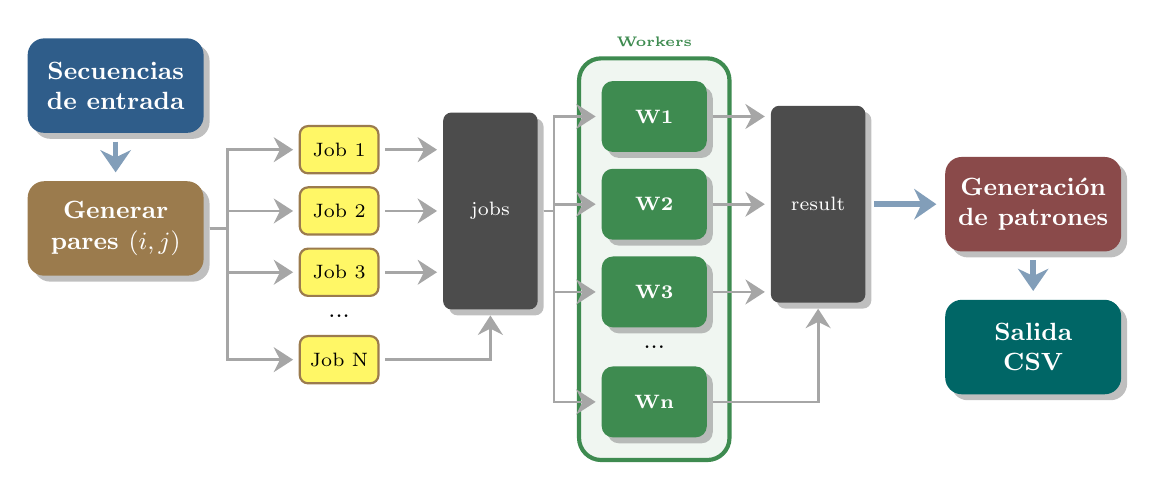
\begin{tikzpicture}[
    node distance=0.8cm and 1.2cm,
    % Estilos para nodos principales
    mainbox/.style={
            rectangle,
            rounded corners=6pt,
            minimum width=2.2cm,
            minimum height=1.2cm,
            text centered,
            text width=2cm,
            font=\bfseries\small,
            text=white,
            drop shadow
        },
    % Estilo para workers
    worker/.style={
            rectangle,
            rounded corners=4pt,
            minimum width=1.2cm,
            minimum height=0.9cm,
            text centered,
            text width=1.1cm,
            font=\scriptsize,
            text=white,
            fill=FormalGreen,
            drop shadow
        },
    % Estilo para jobs
    job/.style={
            rectangle,
            rounded corners=3pt,
            minimum width=1cm,
            minimum height=0.6cm,
            text centered,
            font=\scriptsize,
            text=black,
            fill=yellow!60,
            draw=FormalOrange,
            line width=0.8pt
        },
    % Canales
    channel/.style={
            rectangle,
            rounded corners=3pt,
            minimum width=1.2cm,
            minimum height=2.5cm,
            text centered,
            font=\scriptsize,
            text=white,
            fill=gray!60!black,
            drop shadow
        },
    % Flechas
    arrow/.style={
    -{Stealth[length=7pt,width=9pt]},
    line width=1pt,
    color=gray!70,
    shorten <=2pt,
    shorten >=2pt
    },
    thickarrow/.style={
    -{Stealth[length=8pt,width=11pt]},
    line width=2pt,
    color=FormalBlue!60,
    shorten <=3pt,
    shorten >=3pt
    },
    % Grupo contenedor
    groupbox/.style={
            rectangle,
            rounded corners=8pt,
            draw=#1,
            line width=1.5pt,
            fill=#1!8,
            inner sep=8pt
        }
    ]

    % ========== GENERACIÓN DE JOBS ==========
    \node[mainbox, fill=FormalOrange] (genjobs) {Generar\\pares $(i,j)$};

    % ========== ENTRADA (arriba de genjobs) ==========
    \node[mainbox, fill=FormalBlue, above=0.6cm of genjobs] (secuencias) {Secuencias\\de entrada};

    % Jobs individuales (verticales)
    \node[job, right=1.2cm of genjobs, yshift=1cm] (job1) {Job 1};
    \node[job, below=0.15cm of job1] (job2) {Job 2};
    \node[job, below=0.15cm of job2] (job3) {Job 3};
    \node[below=0.1cm of job3, font=\small] (dots) {...};
    \node[job, below=0.1cm of dots] (jobn) {Job N};

    % ========== CANAL DE JOBS (vertical) ==========
    \node[channel, right=0.8cm of job2] (jobchan) {jobs};

    % ========== WORKERS (verticales) ==========
    \node[worker, right=0.8cm of jobchan, yshift=1.2cm] (w1) {\textbf{W1}};
    \node[worker, below=0.2cm of w1] (w2) {\textbf{W2}};
    \node[worker, below=0.2cm of w2] (w3) {\textbf{W3}};
    \node[below=0.1cm of w3, font=\small] (wdots) {...};
    \node[worker, below=0.1cm of wdots] (wn) {\textbf{Wn}};

    % Grupo de workers
    \begin{scope}[on background layer]
        \node[groupbox=FormalGreen, fit=(w1)(w2)(w3)(wdots)(wn), label={[font=\bfseries\tiny, text=FormalGreen]above:Workers}] (workerpool) {};
    \end{scope}

    % ========== CANAL DE RESULTADOS (vertical) ==========
    \node[channel, right=0.8cm of w2] (resultchan) {result};

    % ========== RECOLECCIÓN ==========
    \node[mainbox, fill=FormalRed, right=1cm of resultchan] (collect) {Generación\\de patrones};

    % ========== SALIDA (abajo de collect) ==========
    \node[mainbox, fill=teal!80!black, below=0.6cm of collect] (output) {Salida\\CSV};

    % ========== FLECHAS ==========
    \draw[thickarrow] (secuencias.south) -- (genjobs.north);

    % Flechas de genjobs a jobs
    \draw[arrow] (genjobs.east) -- ++(0.3,0) |- (job1.west);
    \draw[arrow] (genjobs.east) -- ++(0.3,0) |- (job2.west);
    \draw[arrow] (genjobs.east) -- ++(0.3,0) |- (job3.west);
    \draw[arrow] (genjobs.east) -- ++(0.3,0) |- (jobn.west);

    % Flechas de jobs a canal
    \draw[arrow] (job1.east) -- (jobchan.west |- job1);
    \draw[arrow] (job2.east) -- (jobchan.west |- job2);
    \draw[arrow] (job3.east) -- (jobchan.west |- job3);
    \draw[arrow] (jobn.east) -| (jobchan.south);

    % Flechas de canal a workers
    \draw[arrow] (jobchan.east) -- ++(0.2,0) |- (w1.west);
    \draw[arrow] (jobchan.east) -- ++(0.2,0) |- (w2.west);
    \draw[arrow] (jobchan.east) -- ++(0.2,0) |- (w3.west);
    \draw[arrow] (jobchan.east) -- ++(0.2,0) |- (wn.west);

    % Flechas de workers a resultados
    \draw[arrow] (w1.east) -- (resultchan.west |- w1);
    \draw[arrow] (w2.east) -- (resultchan.west |- w2);
    \draw[arrow] (w3.east) -- (resultchan.west |- w3);
    \draw[arrow] (wn.east) -| (resultchan.south);

    % Flechas finales
    \draw[thickarrow] (resultchan.east) -- (collect.west);
    \draw[thickarrow] (collect.south) -- (output.north);

\end{tikzpicture}

\end{document}
